\documentclass[landscape]{article}
\usepackage{2in1, lscape} 

\usepackage{units} 
\usepackage{parskip} 
\usepackage{xfrac} 
\usepackage[fleqn]{amsmath}
\usepackage{commath}
\usepackage{cancel}
\usepackage{float}
\usepackage{mdwlist}
\usepackage{booktabs}
\usepackage{cancel}
\usepackage{polynom}
\usepackage{caption}
\usepackage{fullpage}
\usepackage{comment}
\usepackage{enumerate}
\usepackage{graphicx}
\usepackage{mathtools} 

\author{}
\title{2014 Major League Baseball}
\date{\today}

\begin{document}

  \maketitle

  \section{Pitching} % (fold)
  
  \section{Definitions} % (fold)

  \subsection{Pitching} % (fold)
  
  \begin{align*}
    ERA  & = \frac{RUNS}{IP/9} \\
    WHIP & = \frac{BB + H}{IP} \\
  \end{align*}

  \subsection{Batting} % (fold)
  \begin{align*}
    SLG &= \frac{1B + (2 \cdot 2B) + (3 \cdot 3B) + (4 \cdot HR)}{AB} \\
    OBP &= \frac{H + BB + HBP}{AB + BB + SF + HBP} \\
    OPS &= OBP + SLG \\
  \end{align*}

  \section{Pitching} % (fold)
  
  \section{Data} % (fold)
  
  \begin{table}[H]
    \centering
    \begin{tabular}{rlrrrrr}
      \toprule
          & Team & ERA   & WHIP  & BB  & SO   & WL \\
      \midrule
      1   & ARI  & 4.260 & 1.340 & 469 & 1278 & 0.395 \\
      2   & ATL  & 3.380 & 1.265 & 472 & 1301 & 0.488 \\
      3   & BAL  & 3.430 & 1.241 & 472 & 1174 & 0.593 \\
      4   & BOS  & 4.010 & 1.324 & 482 & 1213 & 0.438 \\
      5   & CHC  & 3.910 & 1.300 & 504 & 1311 & 0.451 \\
      6   & CHW  & 4.290 & 1.405 & 557 & 1152 & 0.451 \\
      7   & CIN  & 3.590 & 1.237 & 507 & 1290 & 0.469 \\
      8   & CLE  & 3.560 & 1.268 & 464 & 1450 & 0.525 \\
      9   & COL  & 4.840 & 1.439 & 531 & 1074 & 0.407 \\
      10  & DET  & 4.010 & 1.332 & 462 & 1244 & 0.556 \\
      11  & HOU  & 4.110 & 1.335 & 484 & 1137 & 0.432 \\
      12  & KCR  & 3.510 & 1.259 & 440 & 1168 & 0.549 \\
      13  & LAA  & 3.580 & 1.221 & 504 & 1342 & 0.605 \\
      14  & LAD  & 3.400 & 1.206 & 429 & 1373 & 0.580 \\
      15  & MIA  & 3.780 & 1.330 & 458 & 1190 & 0.475 \\
      16  & MIL  & 3.670 & 1.247 & 431 & 1246 & 0.506 \\
      17  & MIN  & 4.570 & 1.391 & 408 & 1031 & 0.432 \\
      18  & NYM  & 3.490 & 1.284 & 509 & 1303 & 0.488 \\
      19  & NYY  & 3.750 & 1.232 & 398 & 1370 & 0.519 \\
      20  & OAK  & 3.220 & 1.145 & 406 & 1244 & 0.543 \\
      21  & PHI  & 3.790 & 1.306 & 521 & 1255 & 0.451 \\
      22  & PIT  & 3.470 & 1.263 & 499 & 1228 & 0.543 \\
      23  & SDP  & 3.270 & 1.225 & 462 & 1284 & 0.475 \\
      24  & SEA  & 3.170 & 1.173 & 463 & 1317 & 0.537 \\
      25  & SFG  & 3.500 & 1.169 & 389 & 1211 & 0.543 \\
      26  & STL  & 3.500 & 1.236 & 470 & 1221 & 0.556 \\
      27  & TBR  & 3.560 & 1.212 & 482 & 1437 & 0.475 \\
      28  & TEX  & 4.490 & 1.413 & 505 & 1110 & 0.414 \\
      29  & TOR  & 4.000 & 1.310 & 490 & 1199 & 0.512 \\
      30  & WSN  & 3.030 & 1.158 & 352 & 1288 & 0.593 \\
      \bottomrule
    \end{tabular}
    \caption{Pitching statistics}
  \end{table}

  \subsection{Graphs} % (fold)
  
  \begin{figure}[H]
    \centering
    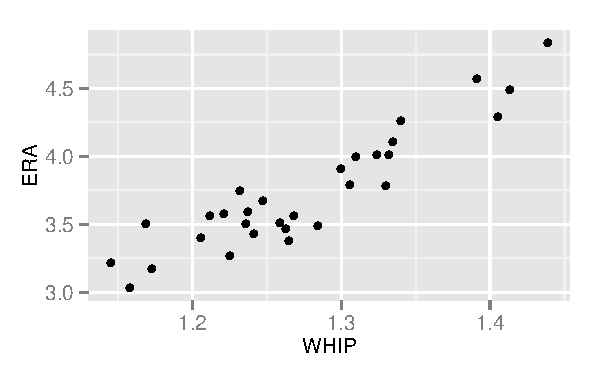
\includegraphics[scale = 0.9]{figures/mlb/whip_vs_era.pdf}
    \caption{WHIP vs. ERA (r = 0.9234)}
  \end{figure}

  \begin{figure}[H]
    \centering
    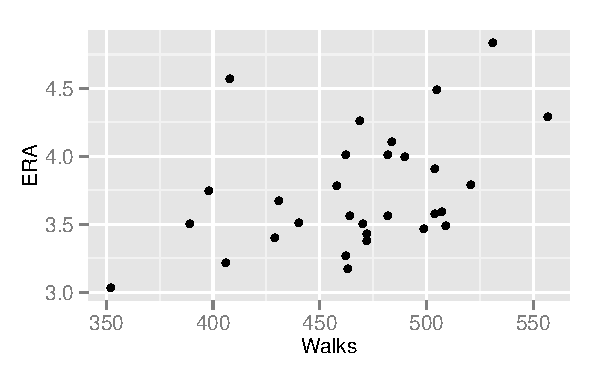
\includegraphics[scale = 0.9]{figures/mlb/bb_vs_era.pdf}
    \caption{Walks vs. ERA (r = 0.4259)}
  \end{figure}

  \begin{figure}[H]
    \centering
    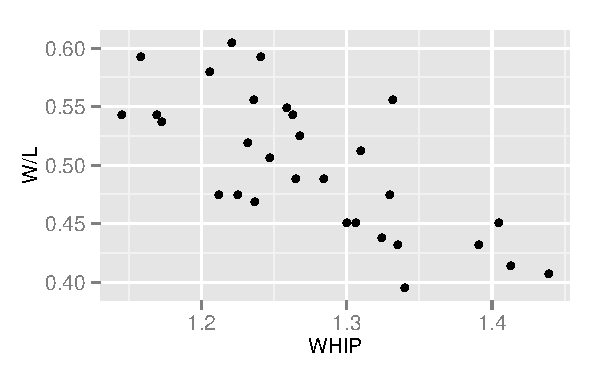
\includegraphics[scale = 0.9]{figures/mlb/whip_vs_wl.pdf}
    \caption{WHIP vs. W/L (r = -0.7276)}
  \end{figure}
  
  \begin{figure}[H]
    \centering
    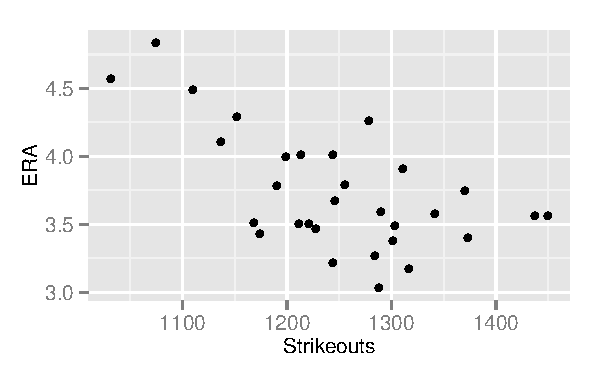
\includegraphics[scale = 0.9]{figures/mlb/so_vs_era.pdf}
    \caption{Strikeouts vs. ERA (r = -0.6126)}
  \end{figure}

  \section{Batting} % (fold)
  
  \subsection{Data} % (fold)
  
  \begin{table}[H]
    \centering
    \begin{tabular}{rlrrrrr}
      \toprule
         & Team  & BB  & BA    & SLG   & OPS   & R/G \\
      \midrule
      1  & ARI   & 398 & 0.248 & 0.376 & 0.678 & 3.800 \\
      2  & ATL   & 472 & 0.241 & 0.360 & 0.665 & 3.540 \\
      3  & BAL   & 401 & 0.256 & 0.422 & 0.734 & 4.350 \\
      4  & BOS   & 535 & 0.244 & 0.369 & 0.684 & 3.910 \\
      5  & CHC   & 442 & 0.239 & 0.385 & 0.684 & 3.790 \\
      6  & CHW   & 417 & 0.253 & 0.398 & 0.708 & 4.070 \\
      7  & CIN   & 415 & 0.238 & 0.365 & 0.661 & 3.670 \\
      8  & CLE   & 504 & 0.253 & 0.389 & 0.706 & 4.130 \\
      9  & COL   & 397 & 0.276 & 0.445 & 0.772 & 4.660 \\
      10 & DET   & 443 & 0.277 & 0.426 & 0.757 & 4.670 \\
      11 & HOU   & 495 & 0.242 & 0.383 & 0.692 & 3.880 \\
      12 & KCR   & 380 & 0.263 & 0.376 & 0.690 & 4.020 \\
      13 & LAA   & 492 & 0.259 & 0.406 & 0.728 & 4.770 \\
      14 & LAD   & 519 & 0.265 & 0.406 & 0.738 & 4.430 \\
      15 & MIA   & 501 & 0.253 & 0.378 & 0.694 & 3.980 \\
      16 & MIL   & 423 & 0.250 & 0.397 & 0.708 & 4.010 \\
      17 & MIN   & 544 & 0.254 & 0.389 & 0.713 & 4.410 \\
      18 & NYM   & 516 & 0.239 & 0.364 & 0.673 & 3.880 \\
      19 & NYY   & 452 & 0.245 & 0.380 & 0.687 & 3.910 \\
      20 & OAK   & 586 & 0.244 & 0.381 & 0.700 & 4.500 \\
      21 & PHI   & 443 & 0.242 & 0.363 & 0.665 & 3.820 \\
      22 & PIT   & 520 & 0.259 & 0.404 & 0.734 & 4.210 \\
      23 & SDP   & 468 & 0.226 & 0.342 & 0.634 & 3.300 \\
      24 & SEA   & 396 & 0.244 & 0.376 & 0.676 & 3.910 \\
      25 & SFG   & 427 & 0.255 & 0.388 & 0.699 & 4.100 \\
      26 & STL   & 471 & 0.253 & 0.369 & 0.689 & 3.820 \\
      27 & TBR   & 527 & 0.247 & 0.367 & 0.684 & 3.780 \\
      28 & TEX   & 417 & 0.256 & 0.375 & 0.689 & 3.930 \\
      29 & TOR   & 502 & 0.259 & 0.414 & 0.736 & 4.460 \\
      30 & WSN   & 517 & 0.253 & 0.393 & 0.714 & 4.230 \\
      \bottomrule
    \end{tabular}
  \end{table}

  \subsection{Graphs} % (fold)
  
  \begin{figure}[H]
    \centering
    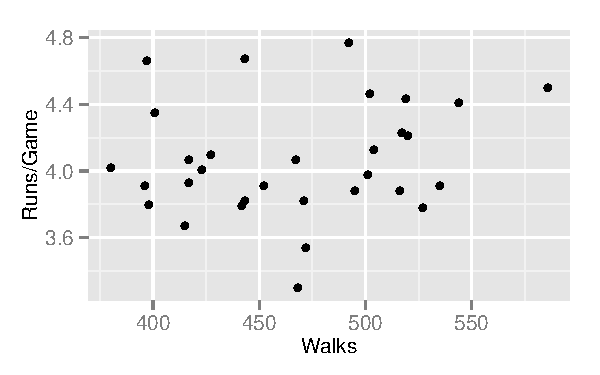
\includegraphics[scale = 0.9]{figures/mlb/bb_vs_rg.pdf}
    \caption{Walks vs. Runs/Game (r = 0.1838)}
  \end{figure}

  \begin{figure}[H]
    \centering
    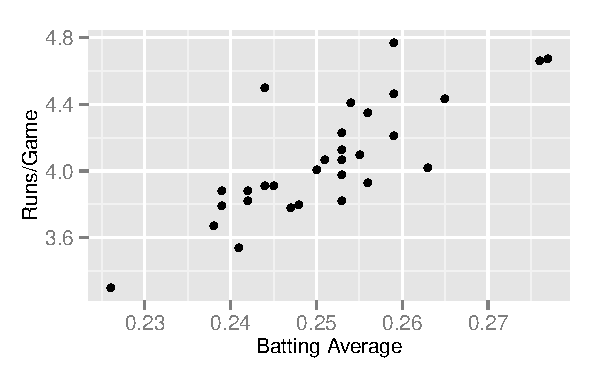
\includegraphics[scale = 0.9]{figures/mlb/ba_vs_rg.pdf}
    \caption{Batting Average vs. Runs/Game (r = 0.7974)}
  \end{figure}

  \begin{figure}[H]
    \centering
    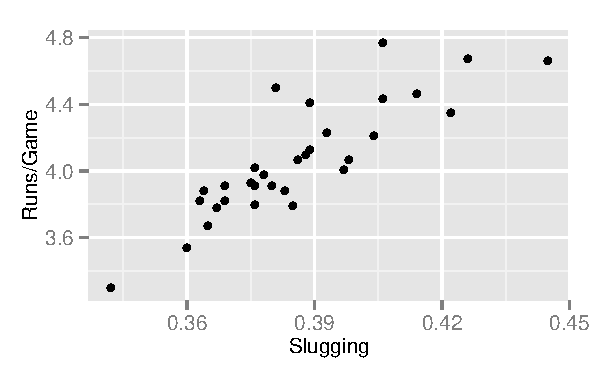
\includegraphics[scale = 0.9]{figures/mlb/slg_vs_rg.pdf}
    \caption{Slugging vs. Runs/Game (r = 0.8568)}
  \end{figure}

  \begin{figure}[H]
    \centering
    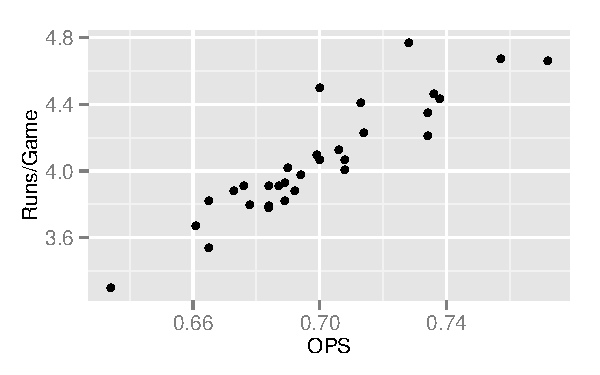
\includegraphics[scale = 0.9]{figures/mlb/ops_vs_rg.pdf}
    \caption{OPS vs. Runs/Game (r = 0.9052)}
  \end{figure}
\end{document}

